\documentclass[tikz,border=5pt]{standalone}
\usepackage{amsmath}
\begin{document}

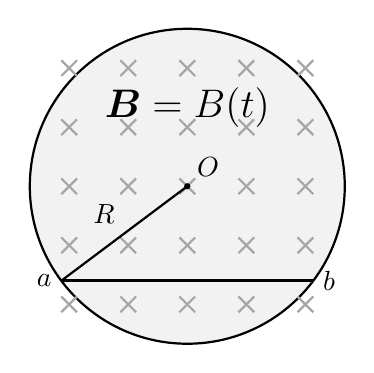
\begin{tikzpicture}[>=stealth]

% 绘制圆形区域
\fill[gray!10] (0,0) circle(2);
\draw[thick] (0,0) circle(2);

% 绘制磁场符号 "×"
\foreach \x in {-1.5,-0.75,0,0.75,1.5}{
  \foreach \y in {-1.5,-0.75,0,0.75,1.5}{
    \draw[gray!70,thick] (\x-0.1,\y-0.1) -- (\x+0.1,\y+0.1);
    \draw[gray!70,thick] (\x-0.1,\y+0.1) -- (\x+0.1,\y-0.1);
  }
}

% 圆心O
\fill (0,0) circle(0.04);
\node[above right] at (0,0) {$O$};

% 绘制半径R
\draw[thick] (0,0) -- (-1.6,-1.2);
\node[above left] at (-0.8,-0.6) {$R$};

% 绘制导线ab
%\draw[line width=1pt] (-1.6,-1.2) -- (1.6,0);
%\draw[line width=4pt,white] (-1.6,-1.2) -- (1.6,-1.2); % 背景层使线段更突出
\draw[line width=1pt] (-1.6,-1.2) -- (1.6,-1.2);

% 标注a, b
\node[left] at (-1.6,-1.2) {$a$};
\node[right] at (1.6,-1.2) {$b$};

% 磁场文字 B = B(t)
\node at (0,1) {\Large$\boldsymbol{B} = B(t)$};

\end{tikzpicture}

\end{document}

